\documentclass{panikzettel}

\usepackage{adjustbox}
\usepackage{tikz}
\usepackage{forest}
\usepackage{tikz-uml}
\usetikzlibrary{positioning,arrows.meta,angles}
\usepackage{wrapfig}
\usepackage{pifont}
\newcommand{\cmark}{\text{\ding{51}}}
\newcommand{\xmark}{\text{\ding{55}}}
\usepackage{lastpage}

\usepackage{listings}
\lstset{
    mathescape=true,
    basicstyle=\ttfamily
}

\newcommand{\defeq}{\vcentcolon =}
\newcommand{\eqdef}{=\vcentcolon}

\title{SWT Panikzettel}
\author{Philipp Schröer, Caspar Zecha, Luca Oeljeklaus,\\Christoph von Oy, ``der Dude''}

\begin{document}

\maketitle

\begin{abstract}%
  Dieser Panikzettel ist über die Vorlesung Softwaretechnik. Er basiert auf dem Foliensatz von Prof. Dr. Bernhard Rumpe aus dem Wintersemester 16/17.	\\
  Dieser Panikzettel ist Open Source. Wir freuen uns über Anmerkungen und Verbesserungsvorschläge auf \url{https://git.rwth-aachen.de/philipp.schroer/panikzettel}.
\end{abstract}

\tableofcontents

\newpage

\section{Einleitung: Don't Panic!}

Es scheint, als hätten selbst die Panikzettel-Autoren Dich verlassen.
\pageref{LastPage} Seiten!
Wer soll das Lernen?
Verzweifle nicht.
Wir haben hier nur etwas anders gemacht als sonst: Wir haben fast alle Stichworte aus der Vorlesung mal erwähnt, von denen man wahrscheinlich für die Klausur was gehört haben sollte.
So hilft dir der Panikzettel auch bei maximal schlechter Vorbereitung.

Die meisten Abschnitte solltest du wahrscheinlich nur ein- oder zweimal gelesen haben, dann hast du wahrscheinlich den Großteil verstanden.
Deinen Fokus solltest du auf die Abschnitte Diagrammtypen (\ref{sec:diagrammtypen}) und Vorgehensmodelle (\ref{sec:vorgehensmodelle}) legen.
Muster (\ref{sec:muster}) werden auch relevant sein.
Generative Softwareentwicklung (\ref{sec:gensoft}) wurde außerdem besonders hervorgehoben.

\section{Diagrammtypen}
\label{sec:diagrammtypen}

\subsection{Aktivitätsdiagramm}
\label{sec:aktivitaetsdiagramm}
\begin{center}
	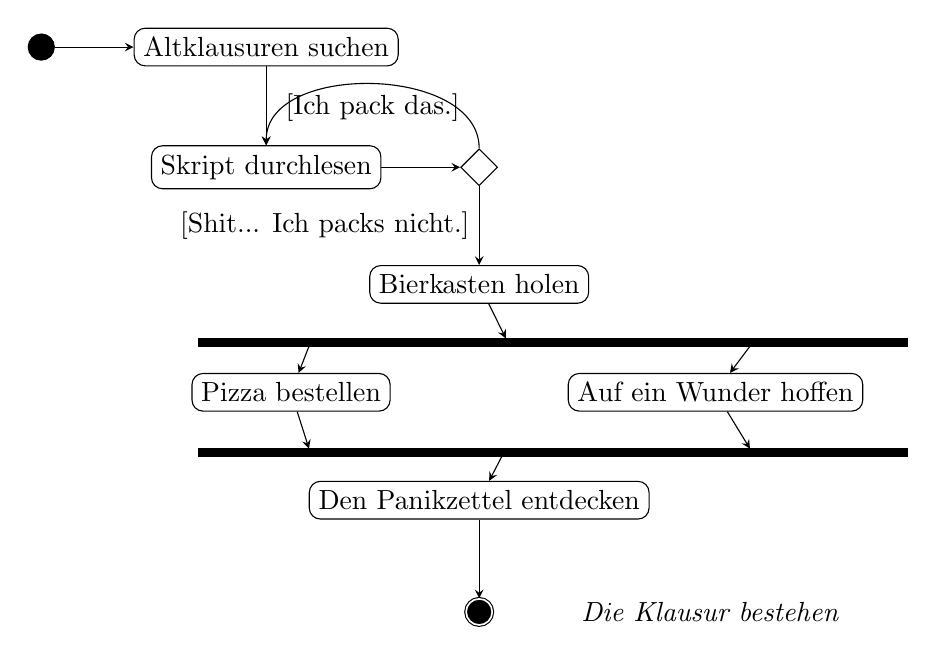
\begin{tikzpicture}[>=stealth,
    every node/.style={shape=rectangle, draw}
                    ]
    % create the nodes
    \node (c0) [shape=circle, fill=black] {};
    \node (c1) [shape=rectangle, right = of c0, rounded corners] {Altklausuren suchen};
    \node (c2) [shape=rectangle, below = of c1, rounded corners] {Skript durchlesen};
    \node (c3) [shape=diamond, right = of c2] {};
    \node (c4) [shape=rectangle, below = of c3, rounded corners] {Bierkasten holen};
    \node (pl) [draw = none, below = of c4]{};
    \node (c5) [shape=rectangle, left = of pl, rounded corners] {Pizza bestellen};
    \node (c6) [shape=rectangle, right = of pl, rounded corners] {Auf ein Wunder hoffen};
    \node (c7) [shape = rectangle, below = of pl, rounded corners]{Den Panikzettel entdecken};
    \node (c8) [shape = circle, fill = black, below = of c7, double]{};
    \node (co) [right = of c8, draw=none]{\textit{Die Klausur bestehen}};
        % connect the nodes
    \draw[->] (c0) edge (c1);
    \draw[->] (c1) edge (c2);
    \draw[->] (c2) edge (c3);
    \draw[->] (c3) to[out=90, in=90] node[below, draw=none]{[Ich pack das.]} (c2);
    \path[->] (c3) edge node[left, draw=none]{[Shit... Ich packs nicht.]}(c4);
    \draw[->] (c4) to (5.9,-3.7);
    \draw[->] (c5) to (3.4,-5.1);
    \draw[->] (c6) to (9,-5.1);
    \draw[->] (3.4,-3.8) to (c5);
    \draw[->] (9,-3.8) to (c6);
    \draw [fill=black] (2, -3.7) rectangle (11, -3.8) ;
    \draw [fill=black] (2, -5.1) rectangle (11, -5.2) ;
    \draw[->] (5.9,-5.1) to (c7);
    \draw[->] (c7) edge (c8);
  \end{tikzpicture}
\end{center}
Diese Zeichnung nennt man \emph{Aktivitätsdiagramm}, man nutzt es um Abläufe und Kausalitäten zu beschreiben.
Rauten ermöglichen es, \emph{Fallunterscheidungen} zu signalisieren, während die schwarzen Balken darauf hindeuten, dass verschiedene Ereignisse \emph{parallel} stattfinden.

\subsection{Use-Case-Diagramm}
\label{sec:usecasediagramm}

\begin{tikzpicture}
  \umlactor{Autoren}
  \umlactor[y=-4]{Korrektoren}
  \umlinherit{Korrektoren}{Autoren}

  \begin{umlsystem}[x=4]{Panikzettel-Server}
    \umlusecase[x=3,name=ansehen]{Ansehen}
    \umlusecase[x=4,y=-3,name=veroeffentlichung]{Veröffentlichung}
    \umlusecase[y=-3,name=korrektur]{Korrektur}
    \umlusecase[x=1.5,y=-1.5,name=upload]{\{abstract\}\\Upload} % TODO: newline
  \end{umlsystem}

  \umlactor[x=13,y=-1]{Studis}

  \umlinherit{veroeffentlichung}{upload}
  \umlinherit{korrektur}{upload}
  \umlassoc{Autoren}{veroeffentlichung}
  \umlassoc{Autoren}{korrektur}
  \umlassoc{ansehen}{Studis}
  \umlassoc{Korrektoren}{korrektur}
  \umlassoc{Korrektoren}{veroeffentlichung}
\end{tikzpicture}

Im obigen Diagramm sieht man ein \emph{Use-Case-Diagramm} für unseren Panikzettel-Server.
Die drei \emph{Akteure} Autoren, Korrektoren\footnote{Weil wir keine Fehler machen, momentan nicht vorhanden.} und Studis interagieren mit dem System und \emph{nehmen an} Use-Cases \emph{teil}.
Die Korrektoren \emph{erweitern} dabei die Akteure Autoren, und nehmen an allen Use-Cases der Autoren teil.
Use-Cases können \emph{spezialisiert} werden, wie etwa Upload durch die Korrektur spezialisiert wird.
Der Use-Case Upload selber ist abstrakt und hält nur Gemeinsamkeiten zwischen anderen Use-Cases fest.

\subsubsection{Use-Case-Beziehung}

Es gibt verschiedene Arten von Use-Case-Beziehungen:

\textbf{Spezialisierung:} (Im Diagramm oben).

\begin{tikzpicture}[scale=0.6,every node/.style={scale=0.6}]
  \umlusecase[name=A]{A}
  \umlusecase[name=B,x=2]{B}
  \umlinherit{B}{A}
\end{tikzpicture}

\textbf{Einbindung:} Use-Case \lstinline{A} ruft \lstinline{B} auf.

\begin{tikzpicture}
  \umlusecase[name=A]{A}
  \umlusecase[name=B,x=4]{B}
  \umlinclude{A}{B}
\end{tikzpicture}

\textbf{Erweiterung:} Use-Case \lstinline{A} wird durch \lstinline{B} erweitert.
Es muss spezielle \emph{extension points} geben, an die die Erweiterungen anknüpfen.
Hier heißt unser extension point ``Korrekturtyp''.

\begin{tikzpicture}
  \umlusecase[name=A,width=3cm]{A\\\textbf{extension point}\\Korrekturtyp}
  \umlusecase[name=B,x=6]{B}
  \umlextend{B}{A}
  \draw (-2.2,0.23) -- (2.2,0.23);
  \node at (4,-0.5) {Korrekturtyp};
\end{tikzpicture}

% TODO
% \subsubsection{Pakete}

%Große Abschnitte von Diagrammen können ``ikonifiziert'' werden.

%\begin{tikzpicture}
%\begin{umlpackage}\node {Halteproblementscheider}; \end{umlpackage}
%\end{tikzpicture}

\subsection{Klassendiagramm}
\label{sec:klassendiagramm}

\begin{tikzpicture}
  \umlinterface[x=4]{Interface}{+String name}{+String getName()}
  \umlclass[y=-4,x=4]{Klasse}{\#Integer int}{+Integer getInt()\\+Integer setInt(Integer int)}
  \umlclass[y=-7]{Unterklasse1}{\#String info}{+String getInfo()}
  \umlclass[y=-7,x=8]{Unterklasse2}{\#Integer zahl}{+Integer getZahl()}
  \umlclass[x=11,y=-2,type=enum]{Color}{RED\\YELLOW\\GREEN}{+TrafficLight switch()\\+boolean canWalk()}

  \umlreal{Klasse}{Interface}
  \umlinherit{Unterklasse1}{Klasse}
  \umlinherit{Unterklasse2}{Klasse}
\end{tikzpicture}

\textbf{Achtung}: In der Vorlesung wird im Gegensatz zum Panikzettel der Name abstrakter Klassen \textit{kursiv} geschrieben.
Es müsste daher im obigen UML-Diagramm \textbf{\textit{Klasse}} statt \textbf{Klasse} heißen.

In diesem Klassendiagramm sind zwei Unterklassen, die von der Klasse $\textit{Klasse}$ erben.
Diese wiederum implementiert das Interface $\textit{Interface}$.
Außerdem ist oben rechts eine Enumerations-Klasse mit drei Konstanten und Funktionen auf diesen Konstanten.

Allgemein kann eine Klasse nur von einer (abstrakten) Klasse erben, aber von mehreren Interfaces.
Ein Interface kann auch von mehreren Interfaces erben.

\subsubsection{Assozationen}
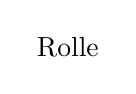
\begin{tikzpicture}
  \umlclass{A}{}{}
  \umlclass[x=10]{B}{}{}

  \umluniassoc[arg1=arg1, mult1=1, arg2=arg2, mult2=*,align2=left]{A}{B}
  \umluniassoc[align2=left]{B}{A}
  %TODO Rolle fehlt
  \node (a)[xshift = 7]{Rolle};
\end{tikzpicture}

Diese Assozation verbindet die Klassen $\textit{A}$ und $\textit{B}$.
Die Assozationsrolle von $\textit{B}$ ist hier als $\textit{arg1}$ (Platzhalter) bzgl. \textit{A} bezeichnet bzw. als \textit{arg2} bezeichnet.
Die Kardinalität (wieviele ``Instanzen''  der Assoziation vorliegen) sieht man unterhalb des Assoziationspfeils und kann folgende Werte annehmen:
\begin{itemize}
  \item genau a: a (oben z.B. 1)
  \item Intervall: a\ldots b
  \item beliebig: * (z.B. im obigen Diagramm)
\end{itemize}

Eine geordnete Assoziation, gekennzeichnet durch $\textit{\{ordered\}}$, gibt an, dass die Reihenfolge der Objekte von Bedeutung ist.

\subsubsection{Qualifizierte Assozation}
Eine Assoziation kann durch einen Qualifikator präzisiert werden.
Der Qualifikator gibt an, nach welchem Typen oder welchem Attribut der Zielklasse die einzelnen Objekte unterschieden werden.
Beispielsweise werden die Personen eines Telefonbuchs nach einem String, dem Namen, voneinander unterschieden. 
Im Klassendiagramm wird der Qualifikator in ein ein Rechteck zwischen Assoziationspfeil und dem Quellrechteck notiert. 

\subsubsection{Komposition}
Eine Komposition ist eine spezielle Form der Assoziation.

\begin{tikzpicture}
  \umlclass[x=2.5]{A}{}{}
  \umlclass[x=0,y=-2]{B}{}{}
  \umlclass[x=5,y=-2]{C}{}{}
  \umlunicompo[arg2=1]{A}{B}
  \umlunicompo[arg2=1]{A}{C}
\end{tikzpicture}

In diesem Klassendiagramm beinhaltet $\textit{A}$ immer genau ein $\textit{B}$  und $\textit{C}$.
Falls $\textit{A}$, $\textit{B}$ oder $\textit{C}$ gelöscht werden, sollten alle Objekte gelöschte werden.

\subsubsection{Sichtbarkeit}
\begin{tabular}{|l|c|c|c|c|}
  \hline
  UML & + & \# & - & \\
  \hline
  Java & public & protected & private & (default)\\
  \hline
  \hline
  Gleiche Klasse & \cmark & \cmark & \cmark & \cmark\\
  \hline
  Andere Klasse (gleiches Paket) & \cmark & UML: \xmark, Java: \cmark & \xmark & \cmark\\
  \hline
  Andere Klasse (anderes Paket) & \cmark & \xmark & \xmark & \xmark\\
  \hline
  Unterklasse (gleiches Paket) & \cmark & \cmark & \xmark & \cmark\\
  \hline
  Unterklasse (anderes Paket) & \cmark & \cmark & \xmark & \xmark\\
  \hline
\end{tabular}

\subsection{Objektdiagramm}
\label{sec:objektdiagramm}
%TODO Klassennamen unterstreichen
\begin{tikzpicture}
  \umlclass{Hans-Rudi:Person}{-vorname = Hans-Rudi \\ -typ = missverstandenes Alien}{}
  \umlclass[x=10]{Hans-Hans:Person}{-vorname = Hans-Hans \\ -typ = fieses baby Alien}{}
  \umlclass[x=5, y=-4]{Hans-Peter:Person}{-vorname = Hans-Peter \\ -typ = süßes baby Alien}{}
  \umlassoc[arg1=vater, arg2=sohn]{Hans-Rudi:Person}{Hans-Hans:Person}
  \umlassoc[arg1=vater, arg2=sohn]{Hans-Rudi:Person}{Hans-Peter:Person}
  \umlassoc[arg1=bruder, arg2=bruder]{Hans-Hans:Person}{Hans-Peter:Person}
\end{tikzpicture}

\emph{Objektdiagramme} sind im Endeffekt ähnlich zu Klassendiagrammen, bis auf die Tatsache, dass man \emph{konkrete Objekte} ohne Methoden und deren Beziehungen darstellt.

\subsection{Sequenzdiagramme}
\label{sec:sequenzdiagramme}

Wir können visualisieren, wie Objekte nacheinander verändert werden.
Dazu verwenden wir \emph{Sequenzdiagramme}.
Zwischen den \emph{Objekten}, für die alle die Zeit gleichmäßig nach unten voranschreitet, werden \emph{Nachrichten} gesendet und empfangen.

\begin{tikzpicture}
  \begin{umlseqdiag}
    \umlobject[class=Studi]{s}
    \umlobject[class=Computer]{c}
    \umlobject[class=PanikzettelServer]{ps}

    \begin{umlcall}[op=getPanikzettel(),return=bild]{s}{c}
      \begin{umlcall}[op=download(),return=panikzettel]{c}{ps}

      \end{umlcall}
    \end{umlcall}
  \end{umlseqdiag}
\end{tikzpicture}

Im obigen Beispiel sehen wir \emph{Aktivierungsbalken}, die vertikalen Balken unter den Objektnamen, die die Lebenszeit eines Objektes darstellen.
Diese Aktivierungsbalken können auch verschachtelt werden.
Objekte können auch explizit erstellt werden, indem die Pfeile direkt auf den Namen (etwa ``s:Studi'') zeigen.
Ebenso kann durch ein Kreuz auf der Linie unter dem Objekt explizite Objektlöschung eingezeichnet werden.

Zwischen den Objekten werden Nachrichten gesendet (oder auch zu sich selbst).
Dabei gibt es vier Pfeilarten: Im Diagramm sind \emph{synchrone} Pfeile zu sehen, wo es keine Verzögerung gibt.
Die Pfeiler mit gestrichelten Linien sind \emph{Returns} und stellen Rückgabewerte von Aufrufen dar.
Außerdem gibt es noch \emph{neutrale} Pfeile, diese stellen keine Festlegung des Kommunikationsmechanismus fest.
\emph{Asynchrone} Pfeile sind für Interaktionen, wo Senden und Empfang unterschiedliche Ereignisse sind (etwa bei SMS-Kommunikation).
~\\~\\
Neutraler Pfeil: 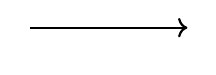
\begin{tikzpicture}
  \tikz [thick] \draw [->] (0,0) -- (2,0);
\end{tikzpicture}

Asynchroner Pfeil (wird schräg eingezeichnet): 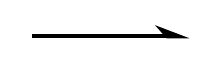
\begin{tikzpicture}
  \tikz [ultra thick] \draw [arrows = {-Stealth[harpoon]}] (0,0) -- (2,0);
\end{tikzpicture}

\subsection{Statecharts}
\label{sec:statecharts}

\emph{Statecharts} beschreiben das Verhalten von Objekten durch endliche  Zustandsübergangsdiagramme (Vgl. endliche Automaten in FOSAP).
Objekte haben einen endlichen Zustandsraum und Transitionen sind markiert mit \lstinline{Ereignis [Bedingung] / Aktion}.
Es gibt immer einen Start- und Endpunkt.

\begin{tikzpicture}
  \umlstateinitial[name=initial]
  \umlstatefinal[name=end,y=-3]
  \begin{umlstate}[name=ready,x=3]{AuctionReady}\end{umlstate}
  \begin{umlstate}[name=open,x=13]{AuctionOpen}
    \begin{umlstate}[name=running]{AuctionRunning}\end{umlstate}
    \begin{umlstate}[name=extended,y=-3]{AuctionExtended}\end{umlstate}
  \end{umlstate}
  \begin{umlstate}[name=finished,y=-3,x=3]{AuctionFinished}\end{umlstate}
  \umltrans[arg={[Uhrzeit: 15:00] / start()}]{ready}{running}
  \umltrans[arg=extend()]{running}{extended}
  \umltrans[arg=finish()]{extended}{finished}
  \umltrans{initial}{ready}
  \umltrans{finished}{end}
\end{tikzpicture}

Wie man am Beispiel von \lstinline{AuctionOpen} sieht, können Zustände verschachtelt werden.

\textbf{Achtung:} Wegen technischer Schwierigkeiten sind hier nicht-hierarchische Zustände auch mit Trennlinien gemalt, dies ist aber in den Folien so nicht vorgesehen!

Zusammengesetze Zustände können ihre eigenen Start- und Endpunkte sowie Transitionen haben, die von allen inneren Zuständen benutzt werden können.

\subsection{Featurediagramme}

\null
\begin{forest}%
  for tree={parent anchor=south,
          child anchor=north,
          l+=1cm,
          fill=white!30,
          delay={content={\strut #1}},
          draw,
          },
  blackcircle/.style={tikz={\node[fill=black!60,inner sep=3pt,circle]at(.north){};}},
  whitecircle/.style={tikz={\node[draw,fill=white!30,inner sep=3pt,circle]at(.north){};}},
  %
  [Auto
    [Radio,whitecircle
      [Radioempfänger,blackcircle]
    ]
    [Gangschaltung,blackcircle
      [Automatik,blackcircle]
      [Manuell,blackcircle]
    ]
    [Felgen,blackcircle
      [Dollar-Felgen,blackcircle]
      [Geschmacklose Felgen,blackcircle]
    ]
  ]
  %
  \foreach \i/\j/\k in {!21/!2/!22}
  {
  \coordinate (A)at (\i.north);
  \coordinate (O)at (\j.south);
  \coordinate (B)at (\k.north);
  \path  (A)--(O)--(B)
  pic [fill=black!60, angle radius=4mm] {angle = A--O--B};
  }
  \foreach \i/\j/\k in {!31/!3/!32}
  {
  \coordinate (A)at (\i.north);
  \coordinate (O)at (\j.south);
  \coordinate (B)at (\k.north);
  \path  (A)--(O)--(B)
  pic [fill=white!30, angle radius=4mm,draw] {angle = A--O--B};
  }
\end{forest}
\par

Legende:
\begin{itemize}
  \item weißer Kreis = optional
  \item schwarzer Kreis = notwendig
  \item weißer Bogen = XOR (genau eins)
  \item schwarzer Bogen = OR (mindestens eins)
\end{itemize}

\subsection{Weitere Diagramme}

Es gibt auch weitere Diagramme aus der Vorlesung, die möglicherweise relevant sein könnten:

\begin{itemize}
  \item \textbf{Blockdiagramm:} Man zeichnet (möglicherweise geschachtelte) Blöcke, die Subsysteme strukturieren. Diese werden durch Linien, die Schnittstellen repräsentieren, verbunden.
  \item \textbf{UML-Implementationsdiagramm:} Die UML-Variante von Blockdiagrammen. Hier werden Namen unterstrichen in die Blöcke geschrieben. Schnittstellen sind Kreise, die mit durchgezogenen Linien an Blöcke angehangen werden. An diese können dann mit den Assoziationen (siehe \ref{sec:klassendiagramm}) andere Blöcke angehangen werden.
  \item \textbf{Konfigurationsdiagramm:} Grobe schematische Zeichnung physikalischer Verteilung von Komponenten.
  \item \textbf{UML-Verteilungsdiagramm:} UML-Variante von Konfigurationsdiagrammen. Komponenten werden durch Linien verbunden. Die Namen haben zusätzlich ``Stereotypen'' wie etwa \lstinline{<<processor>>} oder \lstinline{<<network>>}.
\end{itemize}

\section{Vorgehensmodelle}
\label{sec:vorgehensmodelle}

Es gibt verschiedene inhaltlich bestimmte \emph{Aktivitäten}, die von zeitlich begrenzten \emph{Phasen} zu unterscheiden sind:

\begin{enumerate}
  \item Analyse
  \item Entwurf
  \item Implementierung
  \item Test/Validierung
  \item Deployment (Installation und etwa Schulung)
  \item Evolution inkl. Wartung
\end{enumerate}

\textbf{Das Wasserfall-Modell:} Analyse, Entwurf, Implementierung, Test und Wartung werden nacheinander ausgeführt.
Eignet sich gut für gut im Voraus beschreibbare Projekte.

\textbf{V-Modell:} Zur Qualitätssicherung werden verschiedenen Entwurfsphasen Tests gegenüber gestellt.
Die Entwurfsphasen gehen von oben nach unten, die Tests können dann in umgekehrter Reihenfolge durchgeführt werden.
\begin{enumerate}
  \item Analyse: Abnahmetest
  \item Grobentwurf: Systemtest
  \item Feinentwurf: Integrationstest
  \item Implementierung: Modultest
\end{enumerate}

\textbf{eXtreme Programming:} Evolutionäre Entwicklung in kleinen Schritten.
Tests und Programmcode als Analyseergebnis.
Tests werden oft geschrieben, bevor die Implementierung beginnt.
Für kleine Projekte geeignet.

\textbf{Scrum:} ``Agile Methode''. Inkrementell und iterativ entwickeln und Transparenz, Überprüfung und Anpassung während jedem Zeitpunkt der Entwicklung.
Die drei verschiedenen Aktivitäten, ``Sprint Planning'', ``Sprint Review'' und ``Daily Scrum'' sind zeitlich fest beschränkt.
Ein Sprint dauert i.d.R. 30 Tage und versucht den ``Sprint Backlog'', einen Teil des ``Produkt-Backlogs'' für diesen Monat, zu entwickeln.
Ein sogenanntes ``Burndown-Chart'' visualisiert detailliert den täglichen Fortschritt im Vergleich zum geplanten Fortschritt.

\section{Anforderungsanalyse}

\subsection{Anforderungsermittlung}

Dies ist die erste Hälfte der Analyse und soll vor der Systemmodellierung feststellen, was überhaupt verlangt wird, die Ergebnisse werden im Pflichtenheft festgehalten.

\textbf{Funktionale Anforderung:} Was soll das System tun?
Beispiel: Das System soll Nutzer identifizieren können.

\textbf{Nicht-funktionale Anforderung:} Wie sollen die funktionalen Anforderungen umgesetzt werden?
Unter diese Kategorie fallen verschiedenste Aspekte wie etwa Effizienzanforderungen, Zuverlässigkeitsanforderungen, Anforderungen an den Entwicklungsprozess selber oder juristische oder ethische Anforderungen.

Mischfälle können in in funktionale und nicht-funktionale Anforderungen zerlegt werden.

\textbf{Geschäftsprozess:} Die zeitlich-logische Abfolge von Tätigkeiten zur Erfüllung einer betriebswirtschaftlichen Aufgabe.

Für \emph{grobe} Geschäftsprozessmodelle können wir sehr einfache Flussdiagramme verwenden.
Bei \emph{detaillierten} Geschäftsprozessmodellen werden UML-Aktivitätsdiagramme (\ref{sec:aktivitaetsdiagramm}) verwendet.

\subsection{Anforderungsmodellierung}

\textbf{Anwendungsfall:} Beschreibung einer Klasse von Aktionsfolgen, die ein System ausführen kann, wenn es mit Akteuren interagiert.

\textbf{Akteur:} Beschreibung einer Rolle, die ein Benutzer in Verbindung mit dem System spielt.
Kann auch etwa ein anderes System sein.

Mit Use-Case-Diagrammen (\ref{sec:usecasediagramm}) organisieren wir solche Anwendungsfälle.

\subsection{Modellierung von Aktivitäten}

Eine Verfeinerung der oben genannten Use-Case-Diagramme sind Aktivitätsdiagramme.
Wir verweisen hier wieder auf Abschnitt~\ref{sec:aktivitaetsdiagramm}.

\subsection{Prototyping}

Wir unterscheiden zwischen drei Arten von Prototypen:

\begin{itemize}
  \item Explorativ: Nur zur Analyse verwendet.
  \item Experimentell: Zur Analyse, Entwurf und Implementierung verwendet, aber der experimentelle Prototyp wird selber nicht weiter benutzt.
  \item Evolutionär: Wird weiter zum System ausgebaut.
\end{itemize}

\section{Systemanalyse und Systemmodellierung}

\subsection{Objektorientierte Analyse (OOA)}

Man betrachtet, wie Objekte miteinander interagieren.
Einmal \emph{statisch} mit etwa Klassendiagrammen (\ref{sec:klassendiagramm}) oder \emph{dynamisch} über Objektdiagramme (\ref{sec:objektdiagramm}), welche Zustände und Verhalten betrachten.

\begin{enumerate}
  \item Klassen finden
  \item \textit{Iteration:} \begin{enumerate}
    \item Assoziationen und Aggregationen finden
    \item Attribute finden
    \item Operationen finden, Szenarien finden und überprüfen
  \end{enumerate}
  \item Vererbungsstrukturen finden
  \item Zustandsdiagramme erstellen
  \item Operationen spezifizieren
  \item Strukturen überprüfen
  \item Subsysteme finden
\end{enumerate}

% Wichtige Methoden sind die \emph{Entkopplung von Paketen}, sowie genaue \emph{Zuordnung von Operationen}.

\subsection{Grundlagen der Objektorientierung}

Ein System besteht aus variabel vielen \emph{Objekten}.
Objekte haben definiertes \emph{Verhalten}, \emph{inneren Zustand} und eine eindeutige \emph{Identität}.
Ein Objekt gehört zu einer \emph{Klasse}, die ein Verhaltensschema und Struktur vorgibt.
Klassen können vererbt werden.
\emph{Polymorphie} ermöglicht differenziertes Verhalten von Objekten abhängig davon, zu welcher Unterklasse ein Objekt gehört.

\subsection{CRC-Karten}

Eine Technik zur Gruppenarbeit, wobei auf Karteikarten auf die Vorderseite Ober- und Unterklassen, Verantwortlichkeiten und Mithelfer eingetragen werden.
Auf der Rückseite werden eine natursprachliche Definition sowie alle Attribute notiert.

\subsection{Szenarien}

\textbf{Szenario:} Eine beispielhafte Folge von Interaktionen von Akteuren mit dem System zur Beschreibung eines Anwendungsfalls.
Hier gibt es die Unterscheidung zwischen \emph{Normalfällen} und \emph{Ausnahmefällen}.

Für die Beschreibung von Szenarien verwenden wir Sequenzdiagramme (\ref{sec:sequenzdiagramme}).

\subsection{Modellierung mit Statecharts}

Objektverhalten soll durch einen endlichen Zustandsraum und Transitionen modelliert werden.
Auf die verwendeten Statecharts gehen wir in Abschnitt~\ref{sec:statecharts} genauer ein.

\subsection{Komponenten}

Eine Komponente ist ein Teil einer Software die \emph{explizite Schnittstellen} besitzt, von der Umgebung \emph{unabhängig} ist und \emph{kombinierbar} ist.
Man versucht die Komponenten so zu entwerfen, dass man eine hohe Kohäsion und eine schwache Kopplung erreicht.

\textbf{Kohäsion}: Bezeichnet wie gut eine Programmkomponente eine logische Einheit bildet.\\
\textbf{Kopplung}: Unter Kopplung versteht man, wie stark eine Programmkomponente von anderen abhängt.

\section{Muster}
\label{sec:muster}

\subsection{Entwurfsmuster}

Erfahrung zeigt, dass sich manche Muster in der objektorientierten Softwareentwicklung oft wiederholen.
Dazu haben die Apostel der Softwarearchitektur, die sogenannte ``Gang of Four'', die Bibel ``Design Patterns'' veröffentlicht.

\subsubsection{Adapter/Wrapper}

\begin{wrapfigure}[10]{R}{0pt}
  \begin{tikzpicture}
    % TODO: abstrakt
    \umlclass{Target}{}{
      request()
    }
    \umlclass[x=4]{Adaptee}{}{
        someOtherRequestAPI()
    }
    \umlclass[x=2,y=-3]{Adapter}{}{
        request()
    }
    \umlVHVinherit{Adapter}{Target}
    \umluniassoc{Adapter}{Adaptee}
  \end{tikzpicture}
\end{wrapfigure}

Ein vorgegebenes Objekt (``adaptee'') wird auf eine gewünschte Schnittstelle (``target'') angepasst.
Man kann sich hier vorstellen, eine eigene Liste auf das \lstinline{List}-Interface von Java anzupassen, indem der Adapter Methodenaufrufe des \lstinline{List}-Interface auf die eigene Listen-API überträgt.

Man unterscheidet zwischen Objekt- und Klassenadaptern. % TODO???

\subsection{Analysemuster}

\subsubsection{Exemplar und Beschreibung}

Auch genannt \emph{Item-Item Description}.
Bei vielen Objekten wiederholen sich systematisch immer wieder Werte.

Vergleiche hierzu das Beispiel der \lstinline{Monster}-Klasse, wo in einem fiktiven Spiel jedes Monster, das auftaucht, Instanz dieser Klasse ist.
Wir können die sich immer wieder wiederholenden Daten in der \lstinline{MonsterTyp}-Klasse zusammenfassen, sodass die vielen \lstinline{EinMonster}-Objekte klein und überschaubar bleiben.

\begin{tikzpicture}
  \umlclass{Monster}{
    int HP \\
    Image bild \\
    int angriffspunkte \\
    int verteidigungspunkte
  }{}
  \umlclass[x=5]{EinMonster}{
    int HP
  }{}
  \umlclass[x=10]{MonsterTyp}{
    Image bild \\
    int angriffspunkte \\
    int verteidigungspunkte
  }{}
  \umluniassoc{EinMonster}{MonsterTyp}
\end{tikzpicture}

\subsubsection{Koordinator}

Das Koordinator-Muster fasst Eigenschaften einer Beziehung zwischen zwei Klassen zusammen, die so wirklich nicht zu einer der beiden Klassen allein passen.

Man kann sich etwa die Beziehung ``gebucht haben'' zwischen den Klassen \lstinline{Kunde} und \lstinline{Veranstaltung} vorstellen.
Das Buchungsdatum gehört weder zum Kunden, noch zur Veranstaltung selber, also führt man den Koordinator \lstinline{Buchung} hinzu.

\subsubsection{Abstrakte Oberklasse}

Genau das, was der Titel sagt.
Gemeinsame Eigenschaften/Operationen werden in einer abstrakten Oberklasse zusammengefasst.

\subsubsection{Wechselnde Rolle}

Ein Objekt einer Unterklasse kann in eine andere Unterklasse wechseln.
Man führt nun eine abstrakte Klasse zwischen den beiden Unterklassen und der Oberklasse ein.
Etwa kann ein \lstinline{Student} als Unterklasse von \lstinline{Person} später auch ein \lstinline{Mitarbeiter} werden.

\subsubsection{Komposition}
\label{sec:komposition}

\begin{wrapfigure}[6]{R}{0pt}
  \begin{tikzpicture}
    \umlemptyclass[x=2]{Baum}
    \umlemptyclass[y=-2]{Blatt}
    \umlemptyclass[x=4,y=-2]{Teilbaum}
    \umlinherit{Blatt}{Baum}
    \umlinherit{Teilbaum}{Baum}
    \umluniaggreg[geometry=|-,mult=1..*]{Teilbaum}{Baum}
  \end{tikzpicture}
\end{wrapfigure}

Angenommen, man kann kein Haskell\footnote{\lstinline[language=Haskell]{data Baum = Teilbaum [Baum] | Blatt}. Fertig.} und muss einen Baum implementieren.
Das Kompositionsmuster nutzt eine abstrakte Oberklassen und zwei Unterklassen, das \emph{Blatt}, und das \emph{Kompositum} die in unserem Fall etwa mehrere Bäume speichert.

\subsection{Entwurfsmuster 2} % TODO: Umsortieren?

\subsubsection{Factory Method}

\begin{wrapfigure}[15]{R}{0pt}
  \begin{tikzpicture}
    \umlemptyclass[x=2]{Auto} % TODO: abstract
    \umlemptyclass[y=-2]{Porsche}
    \umlemptyclass[x=4,y=-2]{Opel}
    \umlinherit{Porsche}{Auto}
    \umlinherit{Opel}{Auto}
    \umlclass[x=2,y=-4]{CarFactory}{}{
        create(...): Auto
    }
    \umlHVdep{CarFactory}{Porsche}
    \umlHVdep{CarFactory}{Opel}
  \end{tikzpicture}
\end{wrapfigure}

Bei der Objekterzeugung soll zwischen Varianten (d.h. Unterklassen) gewählt werden, ohne dass der Erzeuger sich darum kümmern muss.
Wir schalten eine \emph{Factory} dazwischen, die sich um das konkrete Erstellen von Objekten kümmert.

Jahrhunderte alte Tradition zwingt uns an dieser Stelle, die klassische Autometapher zu verwenden.
Abhängig davon, ob man Student ist oder nicht, kann hier etwa die \lstinline{CarFactory} entscheiden, welches Auto man bekommt.
Der Nutzer dieser API muss sich dann nicht darum kümmern, wie genau das Auto zusammengebaut wird, denn am Ende des Tages will man doch eigentlich nur Auto fahren, richtig?

\subsubsection{Decorator}

\begin{wrapfigure}[11]{R}{0pt}
  \begin{tikzpicture}
    \umlclass[x=2]{Lautsprecher}{}{
      play(Song song)
    } % TODO: abstract
    \umlclass[y=-3]{Kopfhoerer}{}{
      play(Song song)
    }
    \umlclass[x=4,y=-3]{PartyDecorator}{}{
      play(Song song)
    }
    \umlinherit{Kopfhoerer}{Lautsprecher}
    \umlinherit{PartyDecorator}{Lautsprecher}
    \umluniassoc[geometry=|-,mult=1]{PartyDecorator}{Lautsprecher}
  \end{tikzpicture}
\end{wrapfigure}

Das \emph{Decorator}-Muster erweitert bestehende Schnittstellen um weitere Funktionalität.

In diesem Beispiel betrachten wir \lstinline{Lautsprecher} als abstrakte Komponente.
Ein \lstinline{Kopfhoerer} spielt einen Song, ist also eine konkrete Implementation.
Der \lstinline{PartyDecorator} hingegen \emph{erweitert} lediglich die bestehenden \lstinline{Lautsprecher} so, dass etwa alle Tiefen verstärkt werden und nutzt dann die bestehende \lstinline{play}-Methode.

Auf den ersten Blick erinnert das Klassendiagramm auf der rechten Seite doch sehr an das Muster der Komposition (\ref{sec:komposition}).
Der Unterschied liegt aber darin, nicht einfach mehrere Objekte zu tragen, sondern bestehende Schnittstellen zu erweitern.
Vergleiche hierzu auch die Kardinalität der Assoziationen.

\subsubsection{Singleton}

Es gibt Klassen, von denen es zu jedem Zeitpunkt nur eine Instanz geben sollte.
Man stelle sich etwa eine Datenbankschnittstelle vor, von der es in einem Programm nur eine Instanz geben sollte.
Code sagt mehr als tausend Worte, also hier eine beispielhafte Implementation.

\begin{lstlisting}[language=Java]
public class Database {
  protected static Database instance;
  protected Database() {}
  public static Database getInstance() {
    if (instance == null) instance = new Database();
    return instance;
  }
}
\end{lstlisting}

\lstinline{instance} hält die eindeutige Instanz der Datenbank.
Der Konstruktor wird nicht-öffentlich gemacht.
Eine ``Factory-Method'' \lstinline{getInstance} gibt dann die einzige Instanz zurück (und erstellt sie, wenn sie noch nicht existiert).

Auch praktisch: ``Override Static''.
Um sich die ganzen Aufrufe á la \lstinline{Database.getInstance().doStuff()} zu verkürzen, können auch \emph{statische} Hilfsfunktionen hinzugefügt werden, sodass man dann \lstinline{Database.doStuff()} schreiben kann:

\begin{lstlisting}[language=Java]
  ...
  public static void doStuff() { getInstance().doStuff(); }
  ...
\end{lstlisting}

\subsubsection{Observer}

\begin{wrapfigure}[11]{R}{0pt}
  \begin{tikzpicture}
    \umlclass{Observable}{}{
      addObserver() \\
      deleteObserver() \\
      setChanged() \\
      notifyObservers()
    }
    \umlclass[type=interface,x=5]{Observer}{}{
      update()
    } % TODO: abstract
    \umlclass[y=-3]{Subject}{}{
      getState()
    }
    \umlclass[x=5,y=-3]{ConcreteObserver}{}{
      update()
    }
    \umlinherit{Subject}{Observable}
    \umlinherit{ConcreteObserver}{Observer}
    \umluniassoc[arg=observers,mult=*]{Observable}{Observer}
    \umluniassoc[arg=subjects,mult=*]{ConcreteObserver}{Subject}
  \end{tikzpicture}
\end{wrapfigure}

Wenn mehrere Objekte an Zustandsänderungen eines Objektes interessiert sind, bietet sich das \emph{Observer}-Muster an.

Damit muss das \lstinline{Subject} nichts über die \lstinline{Observer} wissen.

Man kann auch \lstinline{notifyObservers} so modellieren, dass auch nur die Art der Änderung übertragen wird.

\subsection{Architekturmuster für die Struktur}

\subsubsection{Schichten}

Man erinnere sich an das TCP/IP-Modell.

\subsubsection{Blackboard}

\begin{wrapfigure}[15]{R}{0pt}
  \begin{tikzpicture}
    \umlclass{Blackboard}{data}{
      getUpdates() \\
      inspect()
    }
    \umlclass[y=-4]{KnowledgeSource}{eventLoop}{
      execute() \\
      updateBlackboard()
    }
    \umlclass[x=4,y=-2]{Control}{}{
      executeStrategy()
    }
    \umlassoc[mult1=1,mult2=1]{Control}{Blackboard}
    \umlassoc[mult1=*,mult2=1]{KnowledgeSource}{Blackboard}
    \umlassoc[mult2=*]{Control}{KnowledgeSource}
  \end{tikzpicture}
\end{wrapfigure}

Das \emph{Blackboard}-Muster führt eine \emph{Control}-Komponente ein, die verschiedene Strategien auf Daten ausführt.
Diese Daten werden im namensgebenden \emph{Blackboard} gespeichert.
Die ausgeführten Strategien werden \emph{Knowledge Sources} genannt.

Man stelle sich einen Compiler vor, der mit verschiedenen Strategien versucht, den Code zu optimieren.
Manche Ansätze funktionieren, manche nicht.
Hier wären mögliche Knowledge Sources die Optimierungsstrategien.
Die Blackboard-Daten wären die Datenstruktur gegeben, die das Programm darstellt.

% TODO: event loop?

\subsubsection{Proxy}

\begin{wrapfigure}[12]{R}{0pt}
  \begin{tikzpicture}
    \umlclass[x=2]{Subject}{}{
      doStuff()
    } % TODO: abstract
    \umlclass[y=-3]{Proxy}{}{
      doStuff()
    }
    \umlclass[x=4,y=-3]{ConcreteSubject}{}{
      doStuff()
    }
    \umlinherit[geometry=|-]{Proxy}{Subject}
    \umlinherit[geometry=|-]{ConcreteSubject}{Subject}
    \umluniassoc{Proxy}{ConcreteSubject}
  \end{tikzpicture}
\end{wrapfigure}

Aus irgendeinem Grund kann man nicht direkt auf ein Objekt zugreifen.
Möglicherweise liegt das Objekt auf einem anderen Rechner, man will aber das Interface einfach halten und so tun, als wäre es lokal.
Ein \emph{Proxy}-Objekt delegiert Verwendungen des Originals durch die gleiche API wie die des Originals.

So kann der Client jetzt die \lstinline{Subject}-API benutzen und es ist egal, woher genau das Objekt kommt.
Es könnte lokal liegen, als \lstinline{ConcreteSubject} oder auch über den \lstinline{Proxy} am anderen Ende der Welt.

Kann auch für andere Zugriffshürden verwendet werden, wie Sicherheitsprobleme oder einen großen Aufwand.

\subsubsection{Model-View-Controller}

Man teilt ein Programm in drei Teilaspekte strukturell auf: \begin{itemize}
\item \emph{Model:} Kümmert sich nur um die reine Datenhaltung.
\item \emph{View:} Kümmert sich um die Sicht auf Daten, etwa über ein GUI.
\item \emph{Controller:} Kümmert sich um die Benutzerschnittstelle und Modifikation. % TODO: Controller vs View/Model
\end{itemize}

\subsection{Architekturmuster für Netzwerkapplikationen}
Man hat nun ein System, was im Netzwerk läuft.
Es gibt verschiedene Möglichkeiten, die Arbeit zwischen Server(n) und den Clients aufzuteilen

\subsubsection{Zentrales System}
Unintelligente Terminals stellen Anfragen an ein kluges zentrales System.
So z.B. bei Mainframe-Anwendungen: Terminals präsentieren Eingabemasken, der Mainframe errechnet die Ausgabe.
Auch: Rein lokale Anwendungen, hier ist der PC Zentrale und Terminal zugleich.

\subsubsection{Two-Tier Client / Server}
Die Aufgaben werden zwischen Terminal und Client aufgeteilt.
So präsentiert der Client die Oberfläche und enthält Teile der Businesslogik.
Der Server ist Beispielsweise für Datenhaltung und Validierung der Client-Eingaben zuständig.

\subsubsection{Thin vs Fat Client}
\emph{Thin-Clients} zeigen nur die Benutzeroberfläche, ähnlich dem Muster Zentrales System.
Nur minimale Aufgaben, wie das Rendering einer GUI aus einer legacy Terminal-Appliaktion erfolgen auf dem Client.

\emph{Fat-Clients} enthalten Teile oder die gesamte Fachlogik auf dem System und führen eigenständig Berechnungen durch.
Fat-Clients sind also analog zum Muster Two-Tier Client / Server.
Der Server ist hauptsächlich für Datenhaltung zuständig.
Dafür müssen die Clients die Rechenkraft und die Daten haben, um die Berechnungen durchzuführen.
Ebenso müssen tendenziell mehr Patches auf den Clients durchgeführt werden.

\subsubsection{Three-Tier Client / Server}
Hier wird zwischen Anwendungsserver und Datenserver unterschieden.
Gerade für den Datenserver kann Standardsoftware benutzt werden.
Dies ist heute der Standard.
Die Applikationslogik liegt gemischt zwischen Anwendungsserver und Client vor.
Der Anwendungsserver führt bei hinreichend großer Applikation auch Load-Balancing durch. 

\subsubsection{Föderation}
Alle beteiligten Systeme kommunizieren in einem Peer-To-Peer-Netzwerk.

\subsubsection{Cloud Computing}
Die IT-Ressourcen werden abstrahiert.
In der Cloud können Server gemietet werden, aber auch ganze Dienste wie DBs oder Load Balancer.

\emph{IaaS}: Infrastruktur (Server, HDDs) werden von einem Anbieter zur Verfügung gestellt.

\emph{PaaS}: Laufzeitumgebungen, die dynamisch angepasst werden können, werden zur Verfügung gestellt.
Skalierung und Patching wird vom Anbieter übernommen.

\emph{SaaS (Software on demand)}: Anwendungsprogramme und Bibliotheken werden
schlüsselfertig von einem Dienstanbieter online zur Verfügung gestellt.

\subsection{Architekturmuster für die Kommunikation}

\subsubsection{Command}

Wir abstrahieren auszuführende Aktionen nicht als Code, sondern als Daten.
Dafür erstellen wir \emph{Commands}, also Objekte, die ihre Operation ausführen können (und ggf. sogar rückgäng machen können).
\lstinline{CommandProcessor} verwaltet \lstinline{Command}-Objekte.
Ein \lstinline{Controller} stellt die Commands über normale Funktionen zur Verfügung.

\begin{tikzpicture}
  \umlclass{CommandProcessor}{commandList}{
  void do(Command c) \\
  void undo()
  }
  \umlclass[x=6]{Command}{}{
  void do() \\
  void undo() \\
  bool isUndoable()
  }
  \umlclass[y=-4]{Controller}{}{
  study()
  }
  \umlassoc{CommandProcessor}{Controller}
  \umluniassoc[mult2=*]{CommandProcessor}{Command}
  \umlclass[x=6,y=-4]{StudyCommand}{}{
  void do() \\
  void undo() \\
  bool isUndoable()
  }
  \umlinherit{StudyCommand}{Command}
  \umldep[mult1=(erstellt)]{Controller}{StudyCommand}
\end{tikzpicture}

Der \lstinline{CommandProcessor} speichert also alle bisher ausgeführten Commands und kann diese dann rückgängig machen (\lstinline{undo}).
Der Rest des Programmes kann nun im Controller \lstinline{study()} aufrufen, welches einen \lstinline{StudyCommand} erstellt und diesen mit dem \lstinline{CommandProcessor} ausführt.

\subsubsection{Interceptor}

Angenommen, wir wollen einem Webserver modular Features hinzufügen, etwa um vor jedem Aufruf einer Website zu prüfen, ob der Nutzer angemeldet ist.
Die einzelnen Funktionen, die Seiten erstellen, sollen aber sich darum nicht kümmern, ob und wie Zugangschecks gemacht werden.

Wir schalten also einen \lstinline{Interceptor}-Interface dazwischen, der von einem \lstinline{Dispatcher} aufgerufen wird, um etwa ein ``Website-Aufruf-Objekt'' zu bearbeiten.
Der \lstinline{Dispatcher} merkt sich alle \lstinline{Interceptor}s und ruft diese nacheinander auf einem Ereignis auf.

\begin{tikzpicture}
  \umlclass{Dispatcher}{}{
  register(Interceptor) \\
  remove(Interceptor) \\
  dispatch(Event)
  }
  \umlclass[x=6,type=interface]{Interceptor}{}{
    handleEvent(Event)
  }
  \umlclass[x=6,y=-3]{LoginCheckInterceptor}{}{
    handleEvent(Event)
  }
  \umlinherit{LoginCheckInterceptor}{Interceptor}
  \umlassoc[mult2=1..*]{Dispatcher}{Interceptor}
\end{tikzpicture}

Nun kann das Webserver-Framework einfach immer den Dispatcher nutzen und das System kann beliebig erweitert werden, indem zum Dispatcher neue Interceptors registriert werden.

\subsubsection{Client-Dispatcher-Server}
Der Dispatcher kennt die Namen aller Server.
Clients wenden sich an den Dispatcher mit dem Namen des gewünschten Servers, dieser gibt dann die IP / den Domainnamen des Servers zurück.
Hier kann transparent Load-Balancing oder eine Zuweisung zum logisch nächsten Server erfolgen (vgl. CDNs).
Die Kommunikation läuft danach direkt, sodass der Dispatcher kein Bottleneck ist und keine Zeit verloren geht.
Es entsteht allerdings ein Overhead und der Dispatcher wird zum Single-Point-of-Failure.

\subsubsection{Broker}
Broker sind ähnlich zum Client-Dispatcher-Server Muster.
Allerdings wird der gesamte Traffic durch den Broker geleitet.
Wenn der Broker eine lokale Klasse ist, kann durch Remote Procedure Calls Zugriffstransparenz erreicht werden.
Als entfernter Server ähneln sich die Aufgaben mit Client-Dispatcher-Server, wobei nur eine Verbindung, nämlich die zum Broker aufgebaut werden muss.
Allerdings wird der Broker zum Bottleneck des gesamten Systems.
\emph{Broker-Bridge}: Mehrere Broker werden über Bridges vernetzt.

\section{Software- und Systementwurf}

Von einer Anforderungsspezifikation (Pflichtenheft) und einer Funktionalen Spezifikation (Produktdefinition) wollen wir zu genauen Aussagen über eine Implementierung kommen.

Ein guter Entwurf erfüllt die Kriterien der \emph{Korrektheit}, \emph{Verständlichkeit und Präzision}, \emph{Hohe Kohäsion}, \emph{Schwacher Kopplung} zwischen Komponenten.

\subsection{``4+1 Sichten''-Modell aus dem Rational Unified Process}

Bei dem Systementwurf ist eine Gliederung der Betrachtungsaspekte sinnvoll.
Nach Philippe Kruchten ist das ``4+1 Sichten''-Modell:

\begin{itemize}
  \item \textbf{Logische Sicht:} Klassenmodell, Verfeinerung des Analysemodells (Endanwender)
  \item \textbf{Struktursicht:} Subsysteme, Schnittstellen (Programmierung, Wartung)
  \item \textbf{Ablaufsicht:} Prozesse, Koordination (System-Integratoren)
  \item \textbf{Physikalische Sicht:} Komponenten, Hardwaresysteme, Netze (Kommunikation, Verteilung, Auslieferung, Installation)
\end{itemize}

Alle vier Sichten überschneiden sich mit den \textbf{Szenarien} (vgl. Use-Case-Diagramme~\ref{sec:usecasediagramm}).

\subsection{Taktiken im Softwareentwurf}

\subsubsection{Verfügbarkeit}

\textbf{Failure:} Von außen beobachtbarer Fehler eines Systems.
Ggf. resultieren mehrere Faults in einem Failure.

\textbf{Fault:} Intern aufgetretener Fehler.
Kann korrigiert werden oder zum Failure werden.

\textbf{Mean Time to Failure (MTF):} Durchschnittliche Zeit zwischen zwei Failures (ohne Down-Zeiten).

\textbf{Mean Time to Repair (MTR):} Durchschnittliche Zeit zur Reparatur eines Failures.

\textbf{Verfügbarkeit:} Wir rechnen $\frac{\textrm{MTF}}{\textrm{MTF}+\textrm{MTR}}$.

Für die Fehlererkennung (Fault) bieten sich verschiedene Diagnostiken an: \emph{Exceptions}, regelmäßige \emph{Pings/Echos} durch andere Komponenten oder regelmäßige Meldungen der zu prüfenden Komponente selbst (\emph{Heartbeats}).

Aufgetretene Faults können verschieden behandelt werden:
\begin{itemize}
  \item Abstimmen: Redundante Systeme wählen einen Ersatz
  \item Aktive Redundanz: Redundante Komponenten laufen parallel und bei Ausfall wird einfach die Arbeit übernommen.
  \item Passive Redundanz: Bei Ausfall wird eine passive Komponente zwecks Ersatz zu einer aktiven Komponente gemacht.
  \item Spare: Ein Ersatz\emph{system} übernimmt die Arbeit.
\end{itemize}

\section{Implementation}

\subsection{Auswahl der Programmiersprache}

Wählt Haskell.

\subsection{Codingstandards}

% TODO?

\subsection{Datenstrukturen}

Eine Monade ist ein Monoid in der Kategorie der Endofunktoren. % TODO?

\subsubsection{WTFs pro Minute}
Die wichtigste und einzige valide Metrik für guten Code ist ``WTFs pro Minute''.
Leider noch keine SI-Einheit.

\subsubsection{Google Guava}
\label{sec:guava}

\emph{Guava} von Google ist eine Java-Bibliothek, die viele oft vorkommende Schwierigkeiten in Java vereinfacht.

\textbf{Fail Fast:} Hilfsfunktionen übernehmen das Werfen von Exceptions in Fehlerfällen. \\
\lstinline{checkNotNull(x, "x ist null!")} stoppt, wenn \lstinline{x} \lstinline{null} ist, \\
\lstinline{checkArgument(param \%  2 == 0, "param ist nicht gerade!")} ist speziell für die Validierung von Parametern vorgesehen.

\textbf{Optionals:} Objekte, die \lstinline{null} repräsentieren können, oder einen Wert enthalten können.
Wird benutzt, weil man bei \lstinline{null}s immer so viele \lstinline{NullPointerException}s bekommt, während \lstinline{Optional} nette Funktionen bietet, wie etwa \\ \lstinline{myOptional.or("my default value").toString()}.

\textbf{Immutables:} Es gibt nicht veränderliche Implementation der Java-Typen \lstinline{List}, \lstinline{Set}, etc. \lstinline{ImmutableList.of("a", "b", "c").add("x")} würde etwa crashen.

\textbf{Builders:} Um etwa nicht veränderliche Objekte einfacher zu erzeugen, gibt es sogenannte ``Builder'', denen man Einträge hinzufügen und dann aus diesem Builder etwa eine \lstinline{ImmutableList} erstellen kann.

\subsubsection{Vererbung oder Komposition?}

In der Regel sollte man Komposition vor Vererbung wählen.
Hier ist Komposition im einfachen Sinne ``wir speichern dieses Objekt als Attribut'' gemeint, \emph{nicht} als Muster (\ref{sec:komposition}).

% TODO: dependency injection?

\section{Generative Softwareentwicklung}
\label{sec:gensoft}

\textbf{Generative Software Engineering:} Methode der effizienten Generierung von Software mit Modellen wie UML oder einer DSL, um Qualität zu erhöhen und Entwicklungszeit zu senken.

\textbf{Domain Specific Language (DSL):} Eine Sprache für eine spezielle Domäne/einen speziellen Anwendungsbereich.
Es gibt eine graphische Sprache zur Gleisnetzbeschreibung, ``NESTML'', eine Sprache zur Beschreibung von neuronalen Netzen, ``ProNet\textsuperscript{sim}'' zur Modellierung und Simulation von Logistik.

\subsection{MontiCore}

``MontiCore'' ist eine Sprache zur Beschreibung von ``modularen Sprachfragmenten''.
Dazu gibt es auch viele Werkzeuge zur generativen Softwareentwicklung.
MontiCore wird hier an der RWTH entwickelt.
Es gibt verschiedene Komponenten:

\textbf{Freemarker:} Eine Template-Sprache, die Einbettung von Daten in Text erlaubt.
Etwa einen \lstinline{name} einfügen: \lstinline[mathescape=false]|Mein Name ist ${name}|.
Man kann auch komplexere Ausdrücke einfügen oder Template-Variablen zuweisen:
\begin{lstlisting}[mathescape=false]
<#assign person = ${x.getPerson()}>
Mein Name ist ${person.getName()}
\end{lstlisting}

\textbf{Data Explorer (DEx):} Nimmt ein Datemodell und generiert ein Java-Programm mit GUI, Speicher- und Sharingfunktionalität.

\textbf{CD4A:} Eine Modellierungssprache, die ein Klassendiagramm in Textversion mit Java-ähnlicher Syntax ist.
Dies ist das Eingabeformat für DEx.

\adjustbox{valign=t}{\begin{minipage}{.55\textwidth}
\begin{lstlisting}
classdiagram MyBlog {
  class Post {
    String title;
    String content;
    Post parentPost;
  }
  class MediaPost extends Post {
    String category;
    MediaType mediaType;
  }
  enum MediaType {
    DOCUMENT,
    PICTURE;
  }
}
\end{lstlisting}
\end{minipage}}
\hfill
\adjustbox{valign=t}{\begin{minipage}[t]{.45\textwidth}
\lstinline{abstract} ist vor \lstinline{class} möglich.

Es gibt außerdem Syntax für Assoziationen, die im \lstinline{classdiagram}-Block einzufügen sind.
\begin{lstlisting}
association [*] Blog -> Member[*];
\end{lstlisting}

Multiplizitäten optional; default: \lstinline{*}.

Richtungen: \lstinline{->}, \lstinline{<-}, \lstinline{<->}, \lstinline{--}.

Zwei Formen: \lstinline{assocation} und \lstinline{composition}.
\end{minipage}}

Der generierte Java-Code verhindert etwa \lstinline{null}s durch Assoziationen-Verwaltung.
Es werden automatisch für \lstinline{class}-Statements im CD4A-Code vier verschiedene Java-Typen generiert: \lstinline{interface Post}, \lstinline{PostImpl} (erweitert \lstinline{Post}), \lstinline{PostBuilder} (vgl.~\ref{sec:guava}) und ein \lstinline{PostManager} für das Verwalten und Speichern von \lstinline{Post}-Objekten.
Getter und Setter werden auch generiert.

\section{Werkzeuge}

Hier gehen wir weniger ins Detail, denn vieles aus diesem Teil der Vorlesung ist eher wichtig für die Anwendung in der Praxis.

\subsection{Versionierung}

Softwareversionen können und sollten mit Versionsverwaltungssoftware verfolgt werden, sodass jede Änderung, die eine Person macht, protokolliert wird.
Versionsverwaltung ermöglicht außerdem parallele Bearbeitung von Code, Rücknahme von einzelnen Änderungen und Datensicherung.

Wir haben in der Vorlesung ``git'' und ``subversion'' kennengelernt.

\subsection{Build-Automatisierung}

Das Kompilieren von Code sollte automatisiert werden.

``Make'' ist das klassische Werkzeug von 1977. ``Ant'' und ``Maven'' sind neuer und insbesondere für Java gedacht.

\subsection{Projekt- und Wissensmanagement}

``Trac'' ist eine Software, die gleichzeitig als Wiki, Bugreporting-Software, Repository-Browser und mehr dient.

Mit ``Sonar'' können qualitätsrelevante Projektkennzahlen wie Anzahl der Codezeilen oder Tiefe von Vererbungshierarchien überwacht werden.

\subsection{Projektmanagement Plattformen}

Auf \url{https://git.rwth-aachen.de/} findet Ihr nicht nur das Repository dieser Panikzettel, sondern könnt auch gleich eure eigenen Repositories verwalten.

\section{Qualitätsmangement}

\subsection{Prozessintegrierte Qualitätssicherung}

In jeden Übergang zwischen Entwicklungsstadien kann Qualitätssicherung eingebettet werden.

\begin{itemize}
  \item Analyse $\to$ Entwurf: Reviews, Prototyp der Oberfläche
  \item Entwurf $\to$ Implementierung: Reviews, Konsistenzprüfungen, Realisierbarkeitsstudien
  \item Implementierung $\to$ Test: Code-Reviews, Test-Spezifikation, Integrationsplan, Test-Management
  \item Test $\to$ Wartung: Fehlerberichte, Änderungsmangement, Versionsplanung
\end{itemize}

% TODO: CMM?

\subsection{Test und Integration}

\textbf{Testobjekt:} Komponente, die zu testen ist.

\textbf{Testfall:} Satz von Eingaben und Ausgaben.

\textbf{Testdaten:} Daten, die für den Testfall benötigt werden.

\textbf{Testtreiber:} Werkzeug, dass das Testobjekt/den Test aufruft.

\textbf{Platzhalter:} Auch ``stub''/``dummy''. Platzhalter für ein nicht vorhandenes Unterprogramm.

\textbf{Regressionstest:} Erneuter Test, um zu prüfen, dass Änderungen keine neuen Fehler eingeführt haben.

\subsection{Testverfahren}

\textbf{Black box test:} Funktionaler Test nur auf Basis der Spezifikation.
Man verwendet \emph{Äquivalenzklassen}, Tests die das selbe Ergebnis erzeugen, und \emph{Grenzwertttests}, Tests für Randfälle.

\textbf{White box test:} Strukturtest.
Testfälle werden auf Basis des Codes ausgewählt.

\textbf{Kontrollflussorientierter Test.}

\textbf{Datenflussorientierter Test}.

\textbf{Überdeckungsgrad:} Für Tests sollte möglichst jede Zeile Code getestet werden.
Verschiedene Metriken:
\begin{itemize}
  \item Anweisungsüberdeckung: Anteil ausgeführter Anweisungen.
  \item Zweigüberdeckung: Anteil ausgeführter Anweisungen und Verzweigungen.
  \item Pfadüberdeckung: Anteil ausgeführter Programmpfade.
\end{itemize}

\subsection{JUnit}

JUnit ist ein Java Test Framework für automatische Tests.

Methoden und Klassen werden mit Markern markiert.
\begin{itemize}
  \item \lstinline{@Test} markiert eine Testmethode
  \item \lstinline{@Before} wird vor jedem Test ausgeführt
  \item \lstinline{@After} wird nach jedem Test ausgeführt
  \item \lstinline{@BeforeClass} wird vor dem erste Test ausgeführt
  \item \lstinline{@AfterClass} wird nach dem letzten Test ausgeführt
\end{itemize}

\section{Softwareentwicklung}
Im Vergleich zu anderen Ingenieursdisziplinen gibt es bei hier nur reine Entwicklung.
Die Fertigung ist reines Kopieren, da Software ein immaterielles Gut ist.
Dafür ist das Finden und Beheben von Fehlern viel aufwendiger.
Kosten sind fast ausschließlich durch die Personalkosten bestimmt.

Gründe, warum Softwareentwicklung schief gehen kann:
\begin{itemize}
  \item Mangelnde Einbeziehung der Benutzer
  \item Änderung und Unvollständigkeit von Anforderungen
  \item Mangelnde Managementunterstützung
  \item Fehlende Ressourcen
  \item Unklare Ziele und unrealistische Erwartungen
  \item Zeitmangel
\end{itemize}

\end{document}
